\subsubsection{Нет 1}
 
\zadatak Реши
\begin{align*}
\log_{3x+5}(9x^2+8x+8) &> 2.
\intertext{\resenje Ако антилогаритмујемо\index{антилогаритам} обе стране добијамо}
9x^2 + 8x + 8 &> (3x + 5)^2\\
9x^2 + 8x + 8 &> 9x^2 + 30x + 25\\
8x + 8 &> 30x + 25,
\intertext{где је након сређивања}
\noalign{\vskip-6pt}
x&<-\frac{17}{22}
\intertext{Следећи услов је да основа буде већа од 1, то јест}
    3x+5 &> 1\\
    x &> -\frac43,
\end{align*}
одакле следи решење
$$
x \in \ram{\left( -\frac43, -\frac{17}{22} \right)}.
$$
$$
\slika{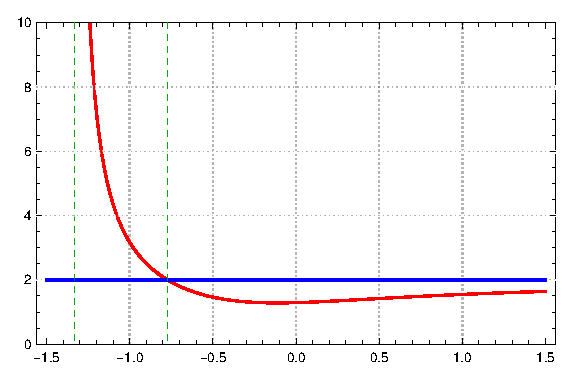
\includegraphics[width=\sirina]{eps/net1.eps}}{$y={\color{red}\log_{3x+5}(9x^2+8x+8)};\,{\color{blue}2}$.}
$$
